\subsubsection{Neural Networks}
There are many variations of neural networks each with its own purpose, however the main type of neural networks I will be focusing on will be feed-forward neural networks and convolutional neural networks. Feed-forward NNs are the most basic type of NNs and also the backbone for many other variations there are. 
\\ \\
Throughout this paper, we will be using the standard notation to avoid any unnecessary confusion
\\
\begin{itemize}
\centering
\item[] 
$n_x$ : Input size \\
$n_y$ : Output size \\
$L$ : Number of layers in Neural Network \\
$n^{[l]}_h$ : Number of hidden units in layer $l$ \\
$m$ : Number of examples in data set \\
$X \in \mathbb{R}^{n_x \times m}$ : Input matrix, can also be referred to as $a^{[0]}$ \\
$x^{(i)} \in \mathbb{R}^{n_x}$ : $i^{th}$ example represented as a column vector \\
$Y \in \mathbb{R}^{n_y \times m}$ : Label matrix for $X$ \\
$y^{(i)} \in \mathbb{R}^{n_y}$ : Output label for the $i^{th}$ example \\
$W^{l} \in \mathbb{R}^{n_h^{l-1} \times n_h^{l}}$ : Weight matrix in layer $l$ \\
$b^{[l]} \in \mathbb{R}^{n^{[l]}_h}$ : Bias vector in layer $l$ \\
$z^{[l]} \in \mathbb{R}^{n^{[l]}_h}$ : Product vector in layer $l$ \\
$g^{[l]}$ : Activation function in layer $l$ \\
$a^{[l]} \in \mathbb{R}^{n^{[l]}_h}$ : Activation vector in layer $l$ \\
$\hat{y} \in \mathbb{R}^{n_y}$ : Predicted output vector. Can also be denoted as $a^{[L]}$
\end{itemize}

Here is an example of a simple Neural Network, with the notation included

\begin{figure}[H]
    \centering
    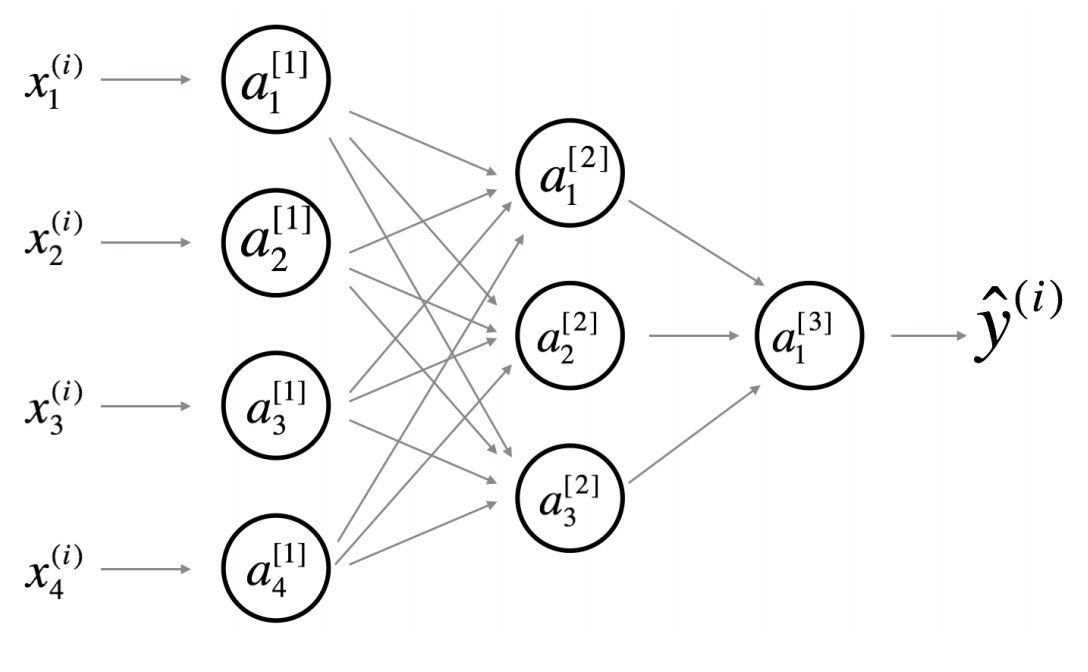
\includegraphics[width=7cm]{Design/Overview/Algorithms/NeuralNetworks/NeuralNetworkDiagram.png}
    \caption{Neural Network Example}
    \label{fig:my_label}
\end{figure}
This network is called a 2 layer network, as it has 1 hidden layer and one output layer.
\subsubsubsection{Forward Propagation} \label{SForwardProp}
Forward Propagation, also referred to as inference, is used to make a prediction given a set of inputs. The inference process for a specific layer in a neural network works as follows:
\begin{enumerate}
    \item The inputs are multiplied by the corresponding weights for that layer and then finally a bias is added, which results with the corresponding $z^{[l]}$ for that layer.
    \item Once the $z^{[l]}$ has been calculated for that layer, the activation's are then calculated using the corresponding $g^{[l]}$ for that layer, which results in $a^{[l]}$.
\end{enumerate}
This process is then repeated throughout every layer until the final layer where the error is calculated.
Using the notation we have established, we can now write this mathematically as: 
\\
\begin{center}
$a^{[l]} = g^{[l]}(z^{[l]})$ \\ 
where $z^{[l]} = W^{[l]}a^{[l-1]} + b^{[l]}$ 
\end{center}

In pseudo-code this may be written as:

\begin{algorithm}[H]
\caption{Dense Forward Propagation Algorithm}\label{DenseForewardProp}
\begin{algorithmic}[1]
\State $net \gets$ Network being used to make prediction
\State $x \gets$ mini-batch
\\
\For{\texttt{each $layer$ in $net$}}
\State $x = Matrix.matmul(layer.w, x) + layer.b$
\State $x = layer.act(x)$
\EndFor
\Return $x$
\end{algorithmic}
\end{algorithm}

Forward propagation for the convolutional layers is the same to that of the dense layers, the only difference being is that instead of matrix multiplication being the operator, the operator is now cross-correlation with both the 3d volumes. In pseudo-code this can be now written as:

\begin{algorithm}[H]
\caption{Convolution Forward Propagation Algorithm}\label{ConvForewardProp}
\begin{algorithmic}[1]
\State $net \gets$ Network being used to make prediction
\State $x \gets$ mini-batch
\State $stridesx \gets$ User Defined
\State $stridesy \gets$ User Defined
\State $padding \gets$ User Defined
\\
\For{\texttt{each $layer$ in $net$}}
\State $x = Volume.conv2d(layer.filter, x, stridesx, stridesy, padding) + layer.b$ (Applying 2d convolution, using x as input and filter as the kernel, with strides = (stridesx, stridesy) )
\State $x = layer.act(x)$
\EndFor 
\Return $x$
\end{algorithmic}
\end{algorithm}
\subsubsubsection{Back-propagation} \label{SBack-propagation}
Back-propagation, is another algorithm with many variations which will be discussed further in the section \ref{Optimisers}. Although there are many techniques for back-propagation they all have the same goal; reduce the error of the network. Therefore the essence of back propagation is to find the correct weight matrix that approximates a given function to an appropriate degree of accuracy in a given interval. Back-propagation, is a \textbf{recursive} algorithm that uses \textbf{memoization} to back-propagates throughout the network to find the \textbf{derivative} of each weight w.r.t (with respect to) a cost. The cost being used, will be set before training and is different for each task.
The notation that will be used in explaining back-propagation will be:

\begin{center}
    $E$ : denotes the error/cost function begin used \\
    $\alpha$ : denotes the learning rate used for back-prop \\
    $\delta^{l}$ : denotes the derivative of the bias matrix $b^{l}$ with respect to the cost function i.e $ \delta^{l} = \frac{\partial E}{\partial b^{l}}$ \\
    $\cdot$ : denotes the hadamard product
\end{center}

The equations, that will be used for back-propagation for a \textbf{Dense} layer will be:
\begin{center}
    $\delta^{l} = ((W^{[l+1]})^{T}\delta^{[l+1]}) \cdot g'^{[l]}(z^{[l-1]})$ \\
    $\frac{\partial E}{\partial W^{l}} = \delta^{l}(a^{[l-1]})^T$ \\
    $\frac{\partial E}{\partial b^{l}} = \delta^{l}$
\end{center}

In summation form this may be written as:

\begin{center}
    $\delta^{l} = \sum_{m} \delta_{m}^{l+1}w_{m,k}$ \\
\end{center}

%write that it took entire night to2 test the network
% explain what cdot represents

The equations, that will be used for back-propagation for a \textbf{Conv} layer will be:
\begin{center}
    $\delta^{l} = \delta^{l+1}_{x,y} \cdot rot_{180^\circ}(w^{l+1}_{x,y}) f'(a^{l}_{x,y})$ \\
    $\frac{\partial E}{\partial W^{l}_{x,y}} = \delta^{l}_{x,y} \cdot f(rot_{180^\circ} (o^{l-1}_{x,y}))$ \\
    $\frac{\partial E}{\partial b^{l}} = \delta^{l}$
\end{center}
In these equations, $w$ denotes a Volume, i.e a lists of matrices with equal dimensions.

In summation form the gradient of the error w.r.t $w^{l}$, in a conv net will be:

\begin{equation*}
    \delta^{l} = rot_{180^\circ} \{\sum_{m=0}^{k_{1} -1} \sum_{n=0}^{k_{2}-1} \delta_{i+m,j+n}^{l+1} w_{m,n}^{l+1}f'(x_{i,j}) \}
\end{equation*}

Finally, the corresponding updates for a layer in the net will be:

\begin{center}
    $W := W - \alpha \frac{\partial E}{\partial W}$ \\
    $b := b - \alpha \frac{\partial E}{\partial b}$
\end{center}
These updates will be applied to every layer in the network on each iteration.

These equations, can be easily derived by extending the chain-rule to matrix multiplication, i.e by using the lemma $\frac{\partial x^Ta}{\partial x} = a$

In pseudo-code this may be written as:
\begin{algorithm}[H]
\caption{Back-propagation Algorithm - Dense Layer}\label{StandardBackpropagation}
\begin{algorithmic}[1]
\State $net \gets$ Network being trained
\State $x \gets$ mini-batch
\State $y \gets$ labels for mini-batch
\\
\State $\hat{y} = forewardPop(x)$
\State $error = \hat{y} - y$
\State $db = [error \times net.gradact(net.last)]$ ($db$ is a list containing the gradient w.r.t the biases for each layer)
\State $dw = [net.layer(-2) \times db.last()]$ (net.layer is a list containing the gradient w.r.t the weight matrices of each layer)
\\
\For{\texttt{each $layer$ in $net$ step -1}}
\State $db.add(matrix.matmul(layer.w.T, deta.last) \cdot net.gradact(layer))$ (Adding the gradient of the loss w.r.t $b^{[layer]}$)
\State $dw.add(layer.act, db.last)$ (Adding the gradient of loss w.r.t  $W^{[layer]}$)
\EndFor
\Return $dw, db$  in the network
\end{algorithmic}
\end{algorithm}

These back-propagation algorithms require a sample of the training data. If each image is used for one back propagation, this is known as stochastic gradient decent, whereas if every image is used in the training sample, then this is known as batch-gradient descent. Batch-gradient descent is more prone to local minimas, however it can take less time to train the network, whereas stochastic gradient descent can take more time but is less prone to locals minimas. Therefore, it is important that the user selects something in between by splitting the training data into different batches each. This is known as mini-batch gradient descent. Therefore, stochastic gradient descent and batch-gradient descent are just special cases for mini-batch gradient descent when $m_b = 1$ and $m_b = m$ where $m_b$ is the mini-batch size, respectively.
\subsubsubsection{Loss-Functions}
The back-propagation algorithms in section \ref{SBack-propagation} relied on a loss function. The loss function, also referred to as the cost function, measures how bad the network is performing. Therefore, the goal of the network is to minimise the loss function, which is done through the use of the back-prop algorithm. This allows the network to learn from the data by minimising the cost function, thus a decreasing loss function implies that the net is learning from the data and a converging loss function implies that the learning is slowing down possibly due to the net having learnt the data, or reaching a global/local minimum. There are a wide array of cost function that are available, however the two most commonly used are: \textbf{soft-max} and 
\textbf{squared error}. 

Minimising a function, is a classic problem in calculus and relies upon the derivative of the function. Furthermore, the back-propagation algorithm in section \ref{SBack-propagation} relies upon the derivative of the loss function. Therefore, it is necessary to be able to compute the derivative of the cost function as it is used to back-propagate throughout the network.

\subsubsubsubsection{Squared-error}
The squared-error loss function measures the average of the sum of the squared error for each data-point.

In mathematical form, the squared-error and its derivative may be written as: 

\begin{center}
    $ E = \frac{1}{2m} \sum^m{(\hat{y}-y)^2}$ \\
    $ \frac{dE}{d\hat{y}} = \hat{y} - y $
\end{center}


These results can be proved by using the chain-rule, i.e using the result $\frac{dy}{dt} = \frac{dy}{dx} \frac{dx}{dt}$

The squared error cost function is commonly used for regression tasks, image-recognition and also used to train many other type of ML models besides neural networks.

\subsubsubsubsection{Soft-max cost function}
The soft-max function, unlike the squared error is most commonly used for multiclass classification. Multiclass classification unlike binary classification, where the data has to belong in one of 2 sets, enables the model to classify objects into more than 2 groups. This is useful for recognition system, where the model is looking out for many different objects at the same time.

Unlike the squared error, softmax works very differently compared to the squared error. The softmax loss function is usually composed of a loss function and an activation function, which is the actual softmax activation function. The loss function being used is usually the cross-entropy loss function.

The softmax activation function works by exponentiating each element in the input vector and then dividing by the sum of this vector. This results in a vector that represents the probability that a given element at an index represent the probability of the image belonging to that class.

Using mathematical notation, the softmax activation function and its respective derivative may then be written as:

\begin{center}
    $ \hat{y} = \frac{e^{z_c}}{\sum_c^{n_y} {e^{z_c}}}$\\
    where $z$ is the product vector and $z_c$ represents the $c_{th}$ item in that vector. An important point to note that since this is the last layer, the length of this vector will be $n_y$ \\
    $ \frac{dE}{d\hat{y}} = \hat{y} * (1-\hat{y}) $
\end{center}

Finally, the cross-entropy loss function works by taking in the vector of probabilities($\hat{y}$) of each class and then applying the natural logarithm to the reciprocal of each element in this vector. Each element is then multiplied by its corresponding $y_i$ which produces a vector, whose elements are then summed up which produces the output of the cross-entropy loss function. 

Using mathematical notation, the cross-entropy activation function and its respective derivative may then be written as:

\begin{center}
    $ E = \sum_c^{n_y} -y_{c}{ log(\hat{y}_{c})} $ \\
    $ \frac{dE}{d\hat{y}} = \hat{y} - y $ \\
    An interesting point to note is that the derivative for the squared error and the cross-entropy loss function is the same.
\end{center}

